\chapter{Higher Derivatives}
\section{Class \texorpdfstring{$C^1$}{C1} Functions}
Open $U$ in $\bbR^m\xrightarrow{f}\bbR^n$. $D(f(a))$ is a linear map $\bbR^m\to \bbR^n$ i.e $D(f(a))\in \mcL(\bbR^m,\bbR^n)$. If $f$ is differentiable at each $a\in U$, then we get a function $Df:{U\to\mcL(\bbR^m,\bbR^n)}$  which maps $a\longmapsto D(f(a))=f'(a)$. We can ask about continuity and differentiability of this map $Df$.

We want to consider $C^1(U)$ functions which are all functions that are differentiable at each $a\in U$ and $Df$ is continuous i.e $C^1(U)=$ Set of continuously differentiable functions
\dfn{$\bs{C^1}$ Functions}{
	$ U$ open in $\bbR^m\xrightarrow{f}\bbR^n$. Suppose $f'(a)$ exists $\forall\ a\in U$ then we get a function \begin{center}
		\begin{tikzcd}[ampersand replacement=\&]
			f: \&[-1cm] U \arrow[r] \& {\mathcal{L}(\mathbb{R}^m,\mathbb{R}^n)} \&[-1cm] {\backsimeq \bbR^{mn}}\\[-0.7cm]
			\& a\arrow[r, maps to] \& f'(a) \&
		\end{tikzcd}
	\end{center}  which maps ${a\longmapsto f'(a)}$. We say $f\in C^1(U)$, "$f$ is continuously differentiable" if $f'(a)$ exists for each $a$ and $f'$ is a continuous function

}
\begin{Theorem}{}{C1 def}
	A function $f:U$ Open in $\bbR^m\to \bbR^n$ is $C^1(U)\iff \lt.\deld{f_i}{x_j}\rt|_a$ exists at each $a\in U$ and are continuous functions
\end{Theorem}
\begin{myproof}
	\subsubsection{If Part:-}
	\begin{enumerate}[label=\bfseries\tiny\protect\circled{\small\arabic*}]
		\item \label{df:1} $a\in U$ Open in $\bbR^m\xrightarrow{f}\bbR^n$ s.t $f(a)=\lt[ \begin{matrix}
					      f_1(a) \\ \vdots\\ f_n(a)
				      \end{matrix} \rt]$, $\lim\limits_{h\to 0}\dfrac{f(a+h)-f(a)-Th}{\|h\|}=0$Matrix of $T$ w.r.t standard basis of $\bbR^m$ and $\bbR^n$ is \[T=  \lt[ \begin{matrix}
					      \lt.\deld{f}{x_1}\rt|_a & \cdots & \lt.\deld{f}{x_m}\rt|_a
				      \end{matrix} \rt]=\lt[ \begin{matrix}
					      \lt.\deld{f_1}{x_1}\rt|_a & \cdots & \lt.\deld{f_1}{x_m}\rt|_a \\
					      \vdots                    & \ddots & \vdots                    \\
					      \lt.\deld{f_n}{x_1}\rt|_a & \cdots & \lt.\deld{f_n}{x_m}\rt|_a
				      \end{matrix} \rt]\]
		\item \label{df:2}$\lim\limits_{x\to v}f(x)=\lt[ \begin{matrix}
					      b_1 \\ \vdots\\ b_n
				      \end{matrix} \rt]\iff \lim\limits_{x\to v}f_I(x)=b_i$ for each $i=1,2,\dots,n$
	\end{enumerate}
	By \ref{df:1} and \ref{df:2}  the proof of forward direction is obvious
	\subsubsection{Only If Part:-}
	If we prove that $f'(a)$ exists for each $a\in U$ then $f'$ is automatically continuous because by \ref{df:1} the matrix of $f'(a)$ must be the Jacobian Matrix and we are given that all entries of this matrix namely the functions $\deld{f_i}{x_j}$ are continuous so apply \ref{df:2}

	\textbf{Another reduction: }We may assume that $n=1$ because this case in general, it follows immediately  that for $f==\lt[ \begin{matrix}
				f_1 \\ \vdots\\ f_n
			\end{matrix} \rt]$, $$f'(a)=\lt[ \begin{matrix}
				f_1(a) \\ \vdots\\ f_n(a)
			\end{matrix} \rt]=\lt[ \begin{matrix}
				\lt.\deld{f}{x_1}\rt|_a & \cdots & \lt.\deld{f}{x_m}\rt|_a
			\end{matrix} \rt]$$Hence $$\dfrac{f(a+h)-f(a)-Th}{\|h\|}=\frac1{\|h\|}\lt( \lt[ \begin{matrix}
				f_1(a+h) \\ \vdots\\ f_n(a+h)
			\end{matrix} \rt]-\lt[ \begin{matrix}
				f_1(a) \\ \vdots\\ f_n(a)
			\end{matrix} \rt]-\lt[ \begin{matrix}
				f_1'(a)h \\ \vdots\\ f_n'(a)h
			\end{matrix} \rt] \rt)$$$\lim\limits_{h\to 0}$ of this $= 0$ because in each slot the limits is 0 by $n=1$ case which we have assumed, and will prove now.
			\nt{Proof of the fact that in case of $n=1$ if $\deld{f_i}{x_j}$ $(j=1,2,\dots,m)$ are continuous functions $U\to \bbR$ then $f'(a)$ exists for each $a\in U$}
			\vspace*{2mm}
			We want to show $f'(a)=\lt[\begin{matrix}
				\lt.\del{f}{x_1}\rt|_a & \cdots & \lt.\del{f}{x_m}\rt|_a
			\end{matrix} \rt]$ i.e $\lim\limits_{h\to 0}\dfrac{f(a+h)-f(a)-Th}{\|h\|}=0$. We want to bound the numerator. Fix $a=\lt[ \begin{matrix}
				a_1 & \cdots & a_m
			\end{matrix} \rt]^T$. Let $h=\lt[ \begin{matrix}
				h_1 & \cdots & h_m
			\end{matrix} \rt]^T$. Now choose $r>0$ such that $B_r(a)\subset U$ and restrict $h$ such that $\|h\|<r$. \[ Th=\sum_j\lt.\deld{f}{x_j}\rt|_ah_j = \lt\langle \underbrace{\lt[\begin{matrix}
					\lt.\del{f}{x_1}\rt|_a \\ \vdots \\ \lt.\del{f}{x_m}\rt|_a
				\end{matrix} \rt]}_{\substack{\parallel \\ q}}, \lt[ \begin{matrix}
				h_1 \\ \vdots \\ h_m
			\end{matrix} \rt] \rt\rangle \]And $f(a+h)-f(a)=f(a_1,h_1,\dots, a_m+h_m)-f(a_1,\dots, a_n)$

	\textbf{Idea:} Bound this in terms of partial derivatives using the mean value theorem (ordinary 1-variable version, which is applicable because each $\del{f}{x_j}$ is continuous)

	\begin{align*}
		f(a+h)-f(a) & = f(a_1+h_1,a_2,\dots, a_m) - f(a)                                                                                                                                                                                       \\
		            & \quad + f(a_1+h_1,a_2+h_2,\dots, a_m) - f(a_1+h_1,a_2,\dots, a_m)                                                                                                                                                        \\
		            & \quad \qquad\qquad\qquad \vdots\qquad\qquad\qquad\qquad\qquad\qquad \vdots                                                                                                                                               \\
		            & \quad + f(a_1+h_1,a_2+h_2,\dots, a_m+h_m) - f(a_1+h_1,a_2+h_2,\dots,a_{m-1}+h_{m-1}, a_m)                                                                                                                                \\
		            & \overset{\text{MVT}}{=} \lt.\del{f}{x_1}\rt|_{v_1}h_1+\lt.\del{f}{x_2}\rt|_{v_2}h_2+\cdots + \lt.\del{f}{x_m}\rt|_{v_m}h_m =\lt\langle \underbrace{\lt[\begin{matrix}
					                                                                                                                                                                     \lt.\del{f}{x_1}\rt|_{v_1} \\ \vdots \\ \lt.\del{f}{x_m}\rt|_{v_m}
				                                                                                                                                                                     \end{matrix} \rt]}_{\substack{\parallel \\ p}}, \lt[ \begin{matrix}
				h_1 \\ \vdots \\ h_m
			\end{matrix} \rt] \rt\rangle
	\end{align*}
	\begin{center}
		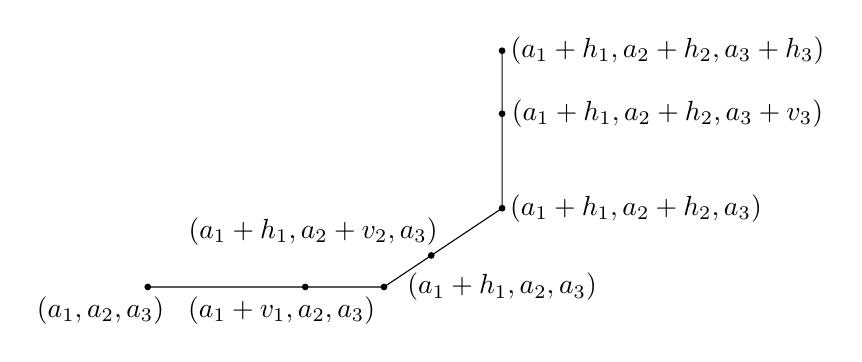
\begin{tikzpicture}
			\draw (0,0) -- (3,0) -- (4.5,1) -- (4.5,3);
			\draw[fill=black] (0,0) node[xshift=-6mm,yshift=-3mm]{$(a_1,a_2,a_3)$} circle (1pt);
			\draw[fill=black] (2,0) node[xshift=-3mm,yshift=-3mm]{$(a_1+v_1,a_2,a_3)$} circle (1pt);
			\draw[fill=black] (3,0) node[xshift=15mm,yshift=-0mm]{$(a_1+h_1,a_2,a_3)$} circle (1pt);
			\draw[fill=black] (3.6,0.4) node[xshift=-15mm,yshift=3mm]{$(a_1+h_1,a_2+v_2,a_3)$} circle (1pt);
			\draw[fill=black] (4.5,1) node[xshift=17mm]{$(a_1+h_1,a_2+h_2,a_3)$} circle (1pt);
			\draw[fill=black] (4.5,2.2) node[xshift=21mm]{$(a_1+h_1,a_2+h_2,a_3+v_3)$} circle (1pt);
			\draw[fill=black] (4.5,3) node[xshift=21mm]{$(a_1+h_1,a_2+h_2,a_3+h_3)$} circle (1pt);
		\end{tikzpicture}
	\end{center}

	Notice that $v_1,v_2,\dots,v_m$ are functions of $h$. Putting together we get
	\begin{align*}
		\dfrac{f(a+h)-f(a)-Th}{\|h\|} & = \frac1{\|h\|} \lt\langle h,\lt[ \begin{matrix}
				                                                                  \lt.\del{f}{x_1}\rt|_{v_1} -	\lt.\del{f}{x_1}\rt|_a \\
				                                                                  \vdots                                              \\
				                                                                  \lt.\del{f}{x_m}\rt|_{v_m}-	\lt.\del{f}{x_1}\rt|_a
			                                                                  \end{matrix} \rt]  \rt\rangle \\
		                              & =\frac1{\|h\|}\|h\|\|p-q\|=\|p-q\|
	\end{align*}
	Showing $\lim\limits_{h\to 0}\|p-q\|=0$ is enough to complete the proof $$ \lim\limits_{h\to 0}\|p-q\|=0\impliedby  p-q\to 0 \text{ as }h\to 0 \impliedby \lt.\del{f}{x_i}\rt|_{v_i} -	\lt.\del{f}{x_i}\rt|_a  \to 0\text{ as }h\to 0 $$ which is true because $\del{f}{x_i}$ is a continuous function. More formally choose $\|h\|<\delta$ s.t $$\lt\|\del{f}{x_i}(b)-	\del{f}{x_1}(a)\rt\| <\frac{\eps}{m}\ \forall \ b\in B_{\delta}(a)$$That ensures $\|p-q\|<\eps$ by triangle inequality.
	\qs{}{ \[ f(x,y)=\begin{cases}
				\frac{xy^2}{xx^2+y^4} & (x,y)\neq (0,0) \\
				0                     & \text{else}
			\end{cases}\]
		\begin{enumerate}
			\item Calculate all directional derivatives in particular $\del{f}{x},\del{f}{y}$
			\item Does $f'(a,b)$ exists at all $a,b\in \bbR$
			\item Is $f$ continuous everywhere
		\end{enumerate}
	}
\end{myproof}

\section{Higher Derivatives and Class \texorpdfstring{$C^k$}{Ck} functions}
Now we want to define class $C^k$  of functions for $k\geq 0$. [Like in 1-Variable case. Usefull for Taylor's theorem].

Now second derivative of $f:U\to\bbR^n$ at $a\in U\subset\bbR^m =$ derivative at $a$ of $f':U\to \mcL(\bbR^m,\bbR^n)\backsimeq \bbR^{mn}$. $\therefore$ $f''(a)$ or $D^2f(a):\bbR^m\to \mcL(\bbR^m,\bbR^n)$. Matrix of $f''(a)$ has $mn$ rows and $m$ columns and equals to $\deld{f'_{pq}}{x_j}$ where $p=1,\dots,n$, $q=1,\dots, m$ and $j=1,\dots, m$

\qs{}{Do $\deld{}{x_l}$ and $\deld{}{x_k}$ commute ?}
\solve{No but actually yes under some good conditions. We discussed here}

If $f''(a)$ exists for all $a\in U$, then  we get a  function $f''$ or $D^2f:U\to \mcL(\bbR^m,\mcL(\bbR^m,\bbR^n))$ which maps $a\mapsto f''(a)$. Dimension of the RHS is $m^2n$. Now we can ask about continuity and differentiability of $f''$

\dfn{$\bs{C^k}$ Functions}{Open $U\subset \bbR^m$, $f:U\to\bbR^n$. Then
	\begin{center}
		\begin{tabular}{rcl}
			$f$ is $C^0$ if        &                                           & $f$ is continuous       \\
			$f$ is $C^1$ if        & $f'(a)$ exists $\forall\ a\in U$ and      & $f'$ is continuous      \\
			$f$ is $C^2$ if        & $f''(a)$ exists $\forall\ a\in U$ and     & $f''$ is continuous     \\
			$\vdots$\hspace{0.5cm} & $\vdots$                                  & \hspace{1cm}$\vdots$    \\
			$f$ is $C^k$ if        & $f^{(k)}(a)$ exists $\forall\ a\in U$ and & $f^{(k)}$ is continuous
		\end{tabular}
	\end{center}

}

\nt{How to understand $\mcL(V,\mcL(U,W))$ where $U,V,W$ are vector spaces. Just set theoretically
	\begin{center}
		\large{\begin{tikzcd}[ampersand replacement=\&]
				\text{Maps}( \& [-1.1cm] A \& [-1.3cm] {,} \& [-1.3cm] \text{Maps}( \& [-1.1cm] B            \& [-0.8cm] {,} \& [-1.1cm] C                       \& [-1.4cm] )) \& [-1cm] \backsimeq      \& [-1.cm] \text{Maps}( \& [-1.1cm] A\times B \& [-0.8cm] {,} \& [-1.1cm] C  \& [-1.4cm] ) \\[-0.7cm]
				\&            \& \downarrow   \&                       \&                       \&              \&                                \&            \&                        \&                      \& \downarrow         \&              \&             \&            \\[-0.7cm]
				\&            \& f(a)         \& :                     \& B \arrow[rr]          \&              \& C \arrow[rrrr, Leftrightarrow] \&            \&                        \&                      \& \phi  \arrow[rr, maps to]   \&              \& {\phi(a,b)}  \&            \\[-0.7cm]
				\&            \&              \&                       \& b \arrow[rr, maps to] \&              \& {\phi(a,b)}                    \&            \&                        \&                      \&                    \&                \&
			\end{tikzcd}}
	\end{center}
	Under this dictionary, maps in $\mcL(V,\mcL(U,W))$ must correspond to some special kind of maps  $V\times U\to W$. }

Hence we can say $\mcL(\bbR^m,\mcL(\bbR^m,\bbR^n))$ is equivalent to the space of maps $\bbR^m\times \bbR^m\to \bbR^n$ which is space of bilinear maps from $\bbR^m\times \bbR^m$ to $\bbR^n$

Component functions of $f':U\to \mcL(\bbR^m,\bbR^n)$ are precisely $\del{f_i}{x_j}$ where $i=1,\dots, n$ and $j=1,\dots, m$. So matrix of $f''(a)$ w.r.t standard basis  of $\bbR^m$ and $\mcL(\bbR^m,\bbR^n)$ will consist of numbers $\lt(\deld{}{x_k}\lt(\deld{}{x_j}f_i\rt)\rt)(a)$. If $f''(a)$ exists   then these are generated to exist. If $f''(a)$ exists at each $a\in U$ then we have the function
\begin{center}
	\begin{tikzcd}
		{f'':} &[-1cm] U\arrow[r] & {\mcL(\bbR^m,\mcL(\bbR^m,\bbR^n))}\ &[-1.2cm] {\backsimeq\text{Space of bilinear maps }\bbR^m\times \bbR^m\to \bbR^n}\\[-0.7cm]
		&[-1cm] a \arrow[r, mapsto] & f''(a)
	\end{tikzcd}
\end{center}

$f''$ is $C^2(U) \overset{\text{definition}}{\iff} f''$ is continuous on $U\iff \deld{}{x_k}\deld{}{x_j}f_i$ are continuous  functions $U\to \bbR$
\begin{Theorem}{}{secdev}
	Let $U$ be open in $\bbR^2$ and $f:U\to \bbR$. $(a,b)\in \bbR$ and $U\supset Q(h,k)=[a,a+h]\times [b,b+k]$. Define \begin{align*}
		\Delta(h,k) & =f(a+h,b+k)-f(a,b+k)-f(a+h,b)+f(a,b)     \\
		            & =[f(a+h,b+k)-f(a+h,b)]-[f(a,b+k)-f(a,b)]
	\end{align*}Then $\exs$ $(s,t)\in $ interior of the rectangle $Q(h,k)$ such that $$\Delta(f,Q)=hk\lt( \del{}{y}\del{}{x}\rt)f(s,t)\coloneqq D_{21}f(s,t)$$
\end{Theorem}
\begin{proof}
	$U(x)=f(x,b+k)-f(x,b)$. Hence $$\Delta(f,Q)=U(a+h)-U(a)$$By $MVT$ we have  $s\in (a,a+h)$ such that \begin{align*}
		\Delta(f,Q) & =hU'(s)=h\lt[ \del{f}{x}(s,b+k)-\del{f}{x}(s,b) \rt]
	\end{align*}Apply $MVT$ again and we get $t\in (b,b+k)$ such that $$\del{f}{x}(s,b+k)-\del{f}{x}(s,b)=k\lt(\del{}{y}\del{}{x}\rt)f(s,t)$$And hence $$\Delta(f,Q)=hk\lt(\del{}{y}\del{}{x}\rt)f(s,t)$$
\end{proof}
\begin{Theorem}{}{}
	Suppose for $f$, $\del{f}{x}$, $\del{f}{y}$, $\del{}{y}\del{}{x}f$ exist everywhere and  $D_{21}f=\del{}{y}\del{}{x}f$ is  continuous  at $(a,b)$. Then $D_{12}f(a,b)=\lt.\del{}{x}\del{}{y}f\rt|_{a,b}$ exists and $$D_{21}f(a,b)=D_{12} f(a,b)$$
\end{Theorem}
\begin{proof}
	Let $\eps>0$ then  continuity of $D_{21}$ means that $\exs$ $\delta>0$  such that  $\forall\ h,k$ with $\max(|h|,|k|)<\delta$ $$\lt| D_{21}f(x,y)-D_{21}f(a,b)\rt|<\eps$$ $\forall\ x,y\in Q(h,k)$
	
	Take $h,k$ as above  and use the  \hyperref[th:secdev]{Theorem \ref{th:secdev}} to find $(s,t)$  such that $\Delta (f,Q)=hkD_{21}f(s,t)$. So $$\lt| \frac{\Delta(f,Q)}{hk}-D_{21}f(a,b) \rt|<\eps \text{ i.e. }
\Bigg| \frac{1}{h}\lt( \frac{f(a+h,b+k)-f(a+h,b)}{k}-\frac{f(a,b+k)-f(a,b)}{k} \rt) -D_{21}f(a,b)\Bigg| <\eps$$
Take limits as $k\to 0$ $$\lt|\frac1h \lt( \del{f}{y}f(a+h,b)-\del{f}{y}f(a,b) \rt)  -D_{21}f(a,b)\rt|<\eps$$As we take limit $h\to 0$ the quantity $\frac1h \lt( \del{f}{y}f(a+h,b)-\del{f}{y}f(a,b) \rt)$ actually exists  and is equal to $D_{21}f(a,b)$ i.e. $\del{}{x}\lt(\del{}{y}f(a,b)\rt)=D_{12}f(a,b)$ exists and is equal to $D_{21}f(a,b)$
\end{proof}
\begin{corolary}{}{}
	If $f$ is  $C^2(U)$ then $D_{21}f=D_{12}f$ at each point of $U$
\end{corolary}
\begin{Theorem}{}{}
	Let $U\subset \bbR^m$ and $f:U\to \bbR^n$ a $C^k$ map  i.e. $k-$th total derivative  $f^{(k)}$ exists and is continuous on $U$  then $$D_{i_1i_2\cdots i_k}f=D_{i_{\sigma(1)}i_{\sigma(2)}\cdots i_{\sigma(k)}}f$$e.g $D_{24714}f=D_{42417}(f)$
\end{Theorem}
\begin{proof}
	May take $m=1$ and work with component real valued functions for $k>2$ keep all but two variables fixed and use earlier result for requisite partial derivative of $f$. Any permutation can be realized as a sequence of transpositions
\end{proof}